\chapter{Running Heat Transport model with BHEs}

\section{Download and compile the source code}
Currently, the BHE feature is developed in a separate branche of OpenGeoSys, to isolate it from changes of the main OGS development. Once this document is finished and the code is fully verified, it will be merged into the OpenGeoSys main branche and released to the public. For interested readers who would like to have a first look, the code can be downloaded from the following link. 
\par
\url{https://github.com/HaibingShao/ogs5-trunk.git}
\par
Most of the changes are kept under the branch \texttt{borehole\_heat\_exchanger}, and they will be constantly merged into the main branch "develop". 

\subsection{Download the source code}
If you are using the Git command line interface, the code can be obtained by typing in the command line prompt as follows.  
\begin{Verbatim}
C:\haibing_working\ogs>git clone https://github.com/HaibingShao/ogs5-trunk.git
\end{Verbatim}
Or, if you prefer a GUI, I personally recommend to use SourceTree on the Windows platform. After a fresh installation of the software SourceTree, the following interface will appear. 
%%
\begin{figure}
\begin{center}
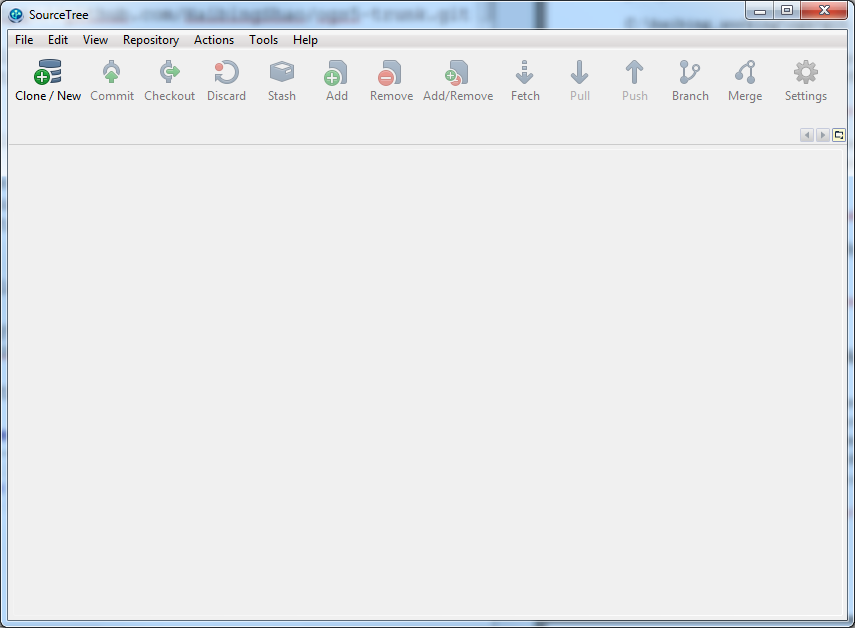
\includegraphics[width=0.8\textwidth]{fig/sourcetree_initial}
\end{center}
\caption{SourceTree window as in the initial stage.}
\label{fig:sourcetree_initial}
\end{figure}
%%
Clicking the button Clone/New in the upper-left corner, you will be asked to give the location of repository. You may use the Github link provided above, or first fork from the above repository and clone from your own repository on Github. 
%%
\begin{figure}
\begin{center}
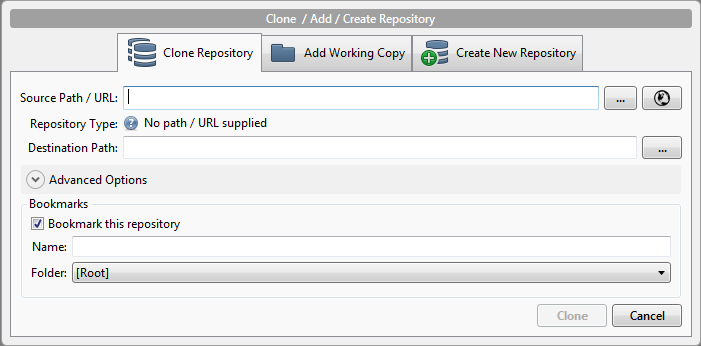
\includegraphics[width=0.6\textwidth]{fig/sourcetree_repo_dialog}
\end{center}
\caption{SourceTree dialog asking for the location of the repository}
\label{fig:sourcetree_repo_dialog}
\end{figure}
%%
After the code has been successfully cloned to your own computer, you will see all history of the development in SourceTree as follows. 
%%
\begin{figure}
\begin{center}
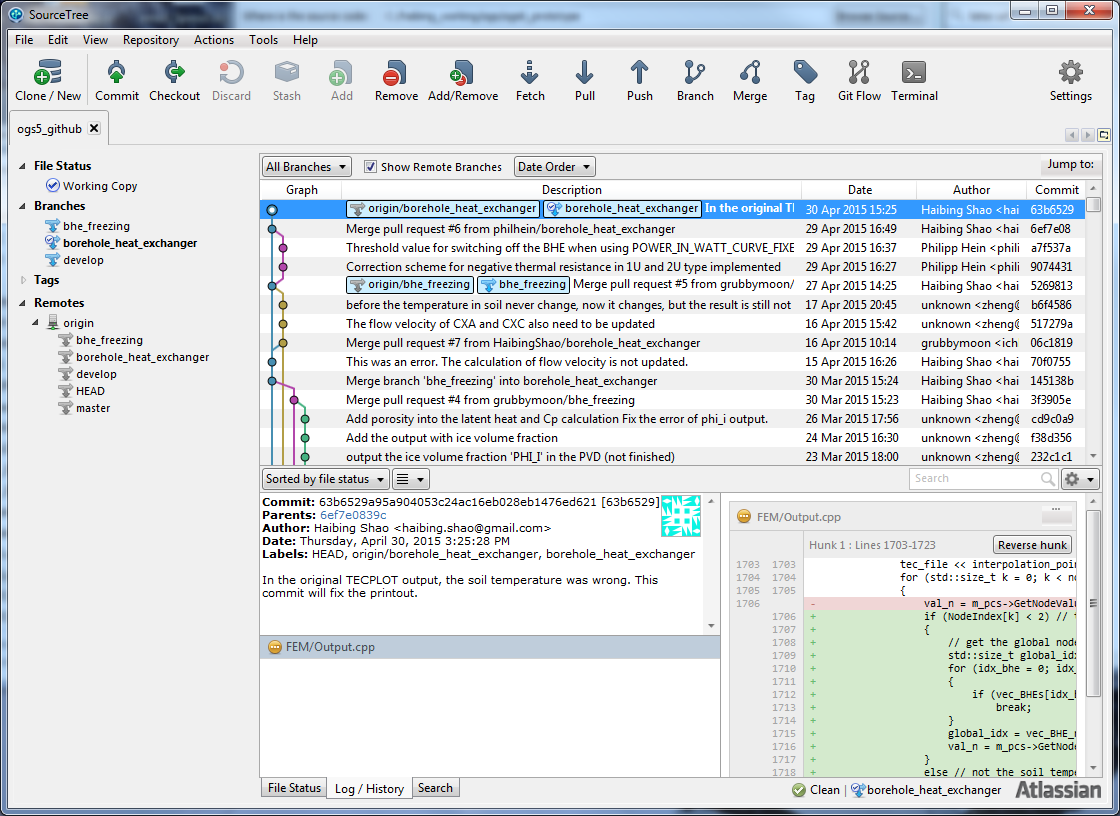
\includegraphics[width=0.8\textwidth]{fig/sourcetree_repo}
\end{center}
\caption{SourceTree window with detailed history of a repository.}
\label{fig:sourcetree_repo}
\end{figure}
%%

\subsection{Using CMake to configure the building project}
Before the compilation of the source code, we need to use the software CMake to generate the configuration and makefiles which are specific to the building environment. Here I am taking CMake version 2.8.12.2 as an example. In the following figure, Cmake GUI was freshly started. First, one needs to define two paths in the CMake GUI. The first one is the folder where the source code of OpenGeoSys is located. The second path refers to the folder where the make files will be generated. 
%%
\begin{figure}
\begin{center}
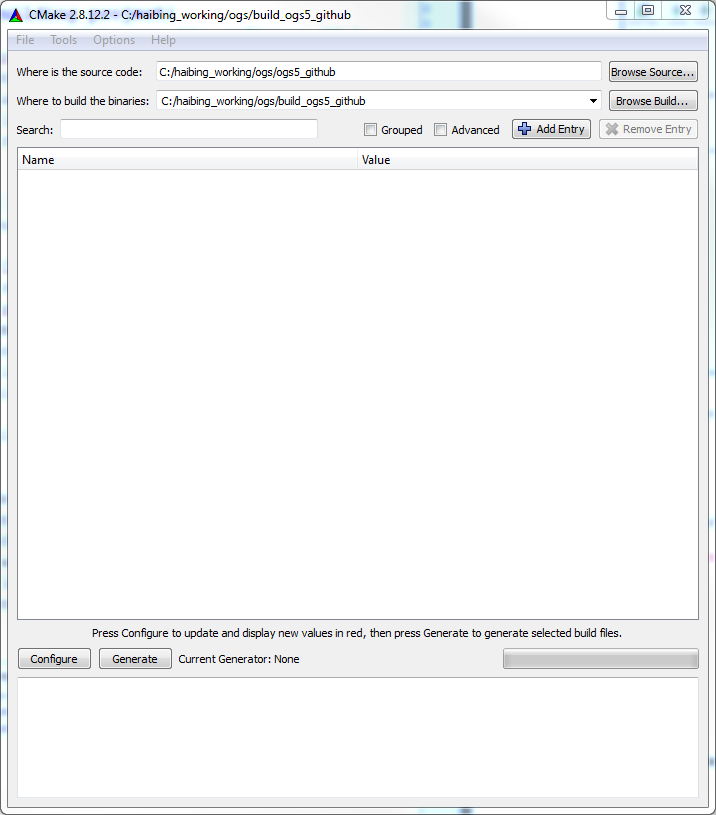
\includegraphics[width=0.6\textwidth]{fig/cmake_initial}
\end{center}
\caption{CMake interface of configuring the build information. }
\label{fig:cmake_initial}
\end{figure}
%%
After clicking on the "Configure" button, CMake will ask several questions, depending on different types of operating system and the compiling tools. In my case, I choose the "Visual Studio 2013 x86" option. Once the configuration has finished, the build options will be demonstrated in the CMake GUI. To build the OpenGeoSys code with BHE features, one only needs to choose the \texttt{OGS\_FEM} option. Finally, once clicking on the "Generate" button, CMake will prepare all makefiles in the build folder. 
%%
\begin{figure}
\begin{center}
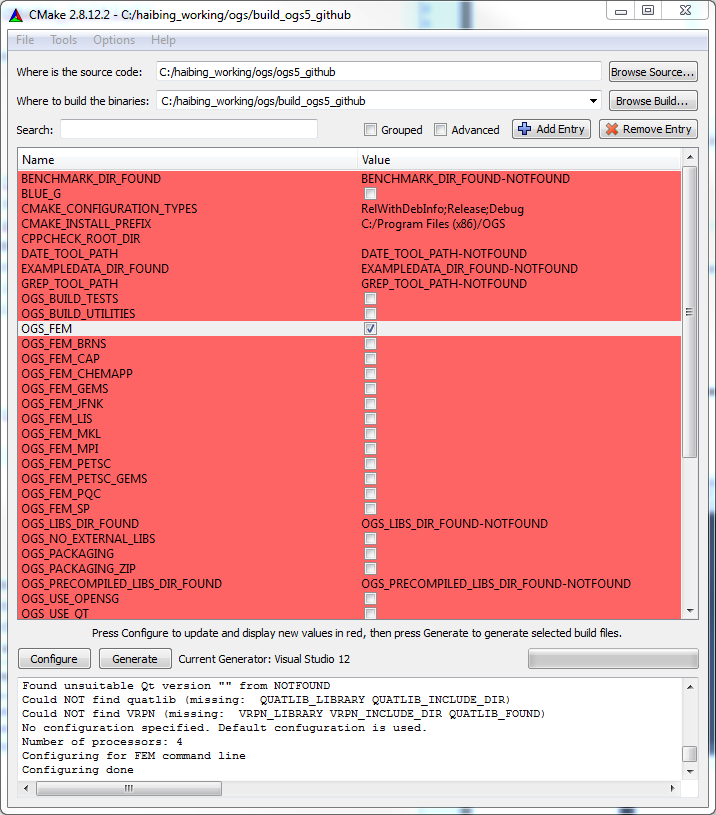
\includegraphics[width=0.6\textwidth]{fig/cmake_configured}
\end{center}
\caption{CMake interface showing different building options. }
\label{fig:cmake_configured}
\end{figure}
%%
\subsection{Compiling the code}
As the author is mainly developing the code with Visual Studio 2013 Express version, the building process will be demonstrated with the same software. Provided the configuration was accomplished by CMake successfully in the previous step, there will be a file named with "OGS.sln" in the build file. Opening this file with Visual Studio will import source code and building configurations into the development environment. 
%%
\begin{figure}
\begin{center}
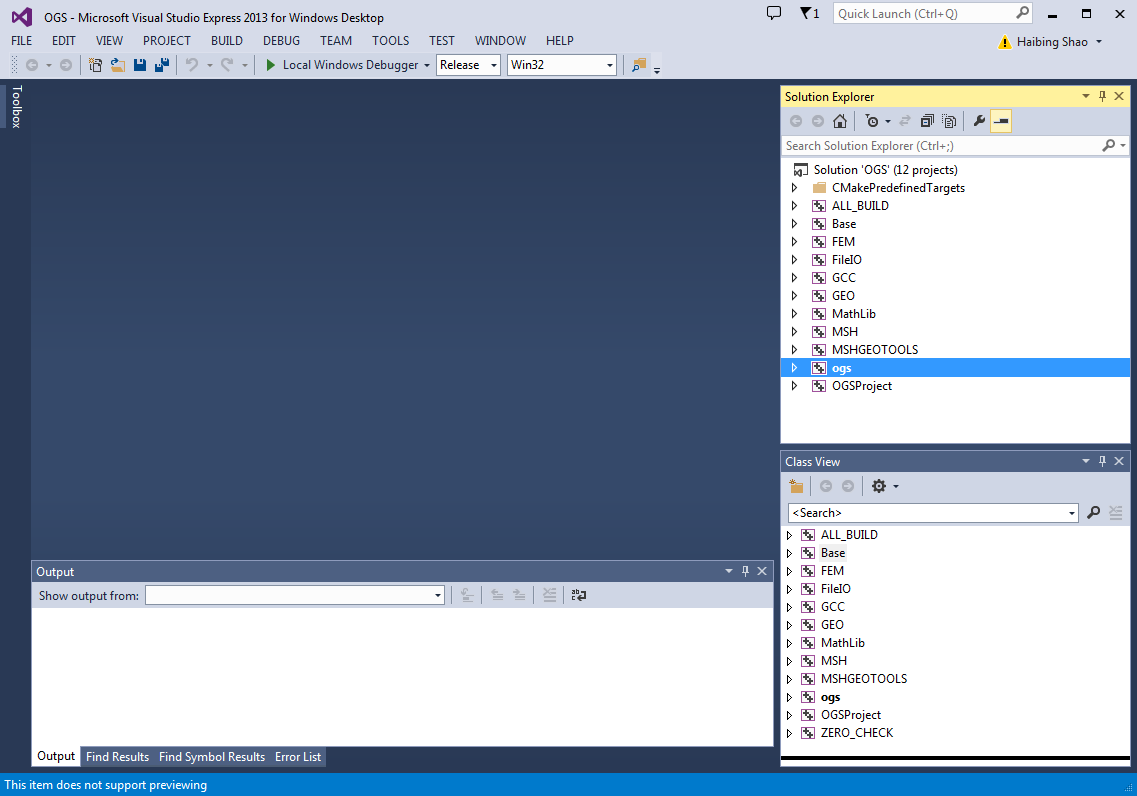
\includegraphics[width=0.8\textwidth]{fig/vs2013exp_ogs}
\end{center}
\caption{Visual Studio interface after opening the OpenGeoSys solution file. }
\label{fig:vs2013exp_ogs}
\end{figure}
%%
To build the source code, choose from the file menu "BUILD", and then click on the first option "Build Solution". It takes a couple of minutes to run the full building process for the first time. After it is finished, the executable files will be found under the bin Debug or bin Release folder, depending on which building mode was chosen. 

\section{Define Heat Transport Process with BHEs}

\section{Geometry of BHEs}

\section{Mesh of BHEs}

\section{Parameters of BHEs}

\section{Output Pipe and Grout Temperatures in the BHEs}

\section{Visualization of the Temperatures}


